\documentclass[a4paper,12pt]{article} % добавить leqno в [] для нумерации слева
\usepackage[a4paper,top=1.3cm,bottom=2cm,left=1.5cm,right=1.5cm,marginparwidth=0.75cm]{geometry}
%%% Работа с русским языком
\usepackage{cmap}					% поиск в PDF
\usepackage[warn]{mathtext} 		% русские буквы в фомулах
\usepackage[T2A]{fontenc}			% кодировка
\usepackage[utf8]{inputenc}			% кодировка исходного текста
\usepackage[english,russian]{babel}	% локализация и переносы
\usepackage{physics}
\usepackage{multirow}
\usepackage{siunitx}

%%% Нормальное размещение таблиц (писать [H] в окружении таблицы)
\usepackage{float}
\restylefloat{table}

\usepackage{graphicx}

\usepackage{caption}
\usepackage{subcaption}

\usepackage{wrapfig}
\usepackage{tabularx}

\usepackage{hyperref}
\usepackage[rgb]{xcolor}
\hypersetup{
	colorlinks=true,urlcolor=blue
}

%%% Дополнительная работа с математикой
\usepackage{amsmath,amsfonts,amssymb,amsthm,mathtools} % AMS
\usepackage{icomma} % "Умная" запятая: $0,2$ --- число, $0, 2$ --- перечисление

%% Номера формул
%\mathtoolsset{showonlyrefs=true} % Показывать номера только у тех формул, на которые есть \eqref{} в тексте.

%% Шрифты
\usepackage{euscript}	 % Шрифт Евклид
\usepackage{mathrsfs} % Красивый матшрифт
\usepackage{pgfplots}
\pgfplotsset{compat=1.9}

%% Свои команды
\DeclareMathOperator{\sgn}{\mathop{sgn}}

%% Не нумеровать секциии
\setcounter{secnumdepth}{0}

%% Перенос знаков в формулах (по Львовскому)
\newcommand*{\hm}[1]{#1\nobreak\discretionary{}
	{\hbox{$\mathsurround=0pt #1$}}{}}

\date{\today}

\begin{document}

\begin{titlepage}
	\begin{center}
		{\large МОСКОВСКИЙ ФИЗИКО-ТЕХНИЧЕСКИЙ ИНСТИТУТ (НАЦИОНАЛЬНЫЙ ИССЛЕДОВАТЕЛЬСКИЙ УНИВЕРСИТЕТ)}
	\end{center}
	\begin{center}
		{\large Физтех-школа прикладной математики и информатики}
	\end{center}
	
	
	\vspace{4.5cm}
	{\huge
		\begin{center}
			{\bf Отчёт о выполнении лабораторной работы 4.6.1}\\
			Интерференция электромагнитных волн миллиметрового диапазона
		\end{center}
	}
	\vspace{1cm}
	\begin{center}
		{\large Соболевский Федор Александрович \\
                    Старокожко Иван Георгиевич \\
			\vspace{0.2cm}
			Б05-111}
	\end{center}
	\vspace{8cm}
	\begin{center}
		  Апрель 2023
	\end{center}
\end{titlepage}

\section{Аннотация}
В данной работе исследовано явление саморепродукции при дифракции света на периодических структурах. При помощи измерения параметров реподукции, а также с помощью геометрического увеличения и измерения пространственного спектра дифракции измерены параметры различных периодических структур: двумерных сеток разных размеров и миры из штриховых решёток. По точности измерений в каждом опыте выявлен наиболее точный метод измерений для каждого типа дифракционных решёток.

\section{Теоретические сведения}
При дифракции плоской световой волны на предмете с периодической структурой наблюдается следующее явление: на некотором расстоянии от предмета вдоль направления распространения волны появляется его изображение, периодически повторяющееся при дальнейшем движении вдоль той же оси. Это явление называется \textit{явлением саморепродукции}.

Запишем выражение для комплексной амплитуды волны, прошедшей через периодическую решётку, в плоскости, отстоящей на расстоянии $z$ от плоскости решётки:
\begin{equation*}
    f(x, z) = \sum c_ne^{i(u_nx + \sqrt{k^2-u_n^2}z)}.
\end{equation*}
Фаза $n$-ой плоской волны плоской волны в плоскости $z = \text{const}$ равна $\varphi_n = \sqrt{k^2 - u_n^2}z\approx kz - \frac{zu_n^2}{2k}$. Сравним набег фазы $n$-ой плоской волны с набегом фазы $\varphi_0$ плоской волны, бегущей вдоль оси $z$: $\varphi_0 = kz$. Получаем разность фаз
\begin{equation}\label{dphi}
    \Delta\varphi_n = \varphi_n - \varphi_0 = \frac{z}{2k}\left(\frac{2\pi}{d}\right)^2n^2 = \pi\frac{\lambda z}{d^2}n^2.
\end{equation}

Рассмотрим плоскость наблюдения, отстоящую от плоскости решётки на расстояние $z_m$, при 
\begin{equation}\label{ZZZ}
    z_m = m\frac{2d^2}{\lambda},\quad z\in\mathbb{N}.
\end{equation}
В этой плоскости из \eqref{dphi} имеем разность $\Delta\varphi_n = 2\pi m n^2$. Получаем, что разность фаз кратна $2\pi$ при любых целых $n$. Аналогично, разность фаз между любыми двумя волнами кратна $2\pi$: $\Delta\varphi_{ij} = 2\pi m(i^2-j^2)$. Получается, что фазовые соотношения между слагаемыми плоскими волнами одинаковы в плоскости решётки и в плоскости наблюдения, откуда следует, что результат интерференции этих волн также одинаков. В этом и заключается суть эффекта саморепродукции.

\section{Экспериментальная установка}
\begin{figure}[h]
    \centering
    \includegraphics[width=0.7\textwidth]{img/setup.png}
    \caption{Схема установки для наблюдения саморепродукции/дифракции}
    \label{fig:setup}
\end{figure}

Хорошим приближением плоской волны в нашем эксперименте служит излучение лазера. Схема экспериментальной установки показана на рис. \ref{fig:setup}. Луч гелий-неонового лазера из генератора оптического квантового генератора (ОКГ) направляется на периодическую структуру О в плоскости $P_0$. В качестве  В плоскостях $P_1$-$P_N$ возникают изображения объекта, которые с помощью линзы Л можно поочерёдно проецировать на экран, установленный в плоскости Э.

Если убрать линзу, то на экране наблюдается картина дифракции луча лазера на периодическом объекты. Экран устанавливается достаточно далеко от объекта, так что лучи, соответствующие различным порядкам дифракции ($\sin \theta_n = n\lambda/d$), разделяются. Измеряя расстояние между дифракционными максимумами, можно определить $\sin \theta_n$ и $d$.

В качестве периодических структур в данной работе используется мира~--- набор различным образом ориентированных одномерных решёток разного период, а также набор из пяти двумерных сеток-решёток. Последние можно рассматривать как пары взаимно перпендикулярных решёток.

\section{Ход работы, результаты}\label{sectionref}

\subsection{Определение периода решёток по их пространственному спектру}
Для первого метода было измерено расстояние между дифракционными максимумами пространственного спектра. Расстояние от экрана до решетки~--- $L = 1282 \text{ мм}$, длина волны лазера здесь и далее~--- $\lambda = 532 \text{ нм}$. Здесь и далее систематическая погрешность измерения длин с помощью линейки равна $\Delta_L = 1$ мм, с помощью нониусного винта линзы~--- $\Delta_x = 0,1$ мм. 

Выразив $\sin\theta_n$ через расстояние до экрана и до $n$-ого максимума, получаем следующее выражение для периода решетки:
\[
d \sin \theta = m \lambda \Longrightarrow d = \frac{L \lambda \cdot N}{X_N}.
\]
Измерения данным методом были проведены для всех двумерных решёток (1-5). Результаты представлены в таблице \ref{tab1}. Погрешность в данном эксперименте можно считать зависящей в основном от систематической. 

\begin{table}[!ht]
    \centering
    \begin{tabular}{|l|l|l|l|l|}
    \hline
        № & $N$ & $X_N$, мм & $x_0$, мм & $d$, см \\ \hline
        1 & 6 & 204 & 34,0 & 0,020$\pm0,003$ \\ \hline
        2 & 4 & 81 & 20,3 & 0,034$\pm0,005$ \\ \hline
        3 & 13 & 148 & 11,4 & 0,0600$\pm0,003$ \\ \hline
        4 & 15 & 90 & 6,0 & 0,114$\pm0,004$ \\ \hline
        5 & 35 & 150 & 4,3 & 0,159$\pm0,006$ \\ \hline
    \end{tabular}
    \caption{Результаты измерения периодов решёток по пространственному спектру}
    \label{tab1}
\end{table}

\subsection{Определение периода решеток по изображению, увеличенному с помощью линзы}
Для второго метода в схему была добавлена собирающая линза, создающая увеличенное изображение на экране. При помощи проволчки, то есть непериодического объекта, найдено первое изображение. Размеры изображений могут быть найдены из формулы увеличения:
\[
d = D \frac ab,
\]
где $a$~--- расстояние до линзы, $b$~--- до экрана. Результаты измерения периодов представлены в таблице \ref{tab2}. Здесь вклад в погрешность вносит также усреднение при расчёте $D$. Также отметим, что в силу мелкости картины не удалось измерить период данным способом для решёток 1 и 2.
\begin{table}[!ht]
    \centering
    \begin{tabular}{|l|l|l|l|}
    \hline
        № & $X_N$, мм & $x_0$, мм & $d$, см \\ \hline
        3 & 51 & 1,8 & 0,089$\pm0,012$ \\ \hline
        4 & 49 & 2,9 & 0,140$\pm0,018$ \\ \hline
        5 & 41 & 3,2 & 0,153$\pm0,022$ \\ \hline
    \end{tabular}
    \caption{Результаты измерения периодов решёток по геометрическому изображению}
    \label{tab2}
\end{table}

\subsection{Исследование эффекта саморепродукции с помощью сеток}
Далее для каждой решетки измерена зависимость координаты саморепродуцированного изображения от его номера. По коэффициенту зависимости можно найти период решетки:
\[
d = \sqrt{ \frac{k\lambda}{2} }
\]
Результаты представлены в таблице \ref{tab3}. Здесь в погрешность измерений входит случайная ошибка метода наилучшей прямой. Графики зависимостей изображены на рис.~\ref{fig:plot} (там же изображены графики для решёток миры, см. далее).

\begin{table}[!ht]
    \centering
    \begin{tabular}{|l|l|l|l|l|l|l|l|l|l|}
    \hline
        № & 0 & 1 & 2 & 3 & 4 & 5 & 6 & k, мм & d, см \\ \hline
        3 & 37,45 & 41,2 & 44,1 & 48,2 & 50,7 & 54,95 & 56,3 & 3,24 & 0,093$\pm0,011$ \\ \hline
        4 & 37,2 & 42,05 & 50,65 & 57,375 & 64,1 & - & - & 6,91 & 0,136$\pm0,016$ \\ \hline
        5 & 37,6 & 48,45 & - & - & - & - & - & 10,85 & 0,170$\pm0,035$ \\ \hline
    \end{tabular}
    \caption{Результаты измерения периодов решёток по репродукции}
    \label{tab3}
\end{table}

\begin{figure}[H]
    \centering
    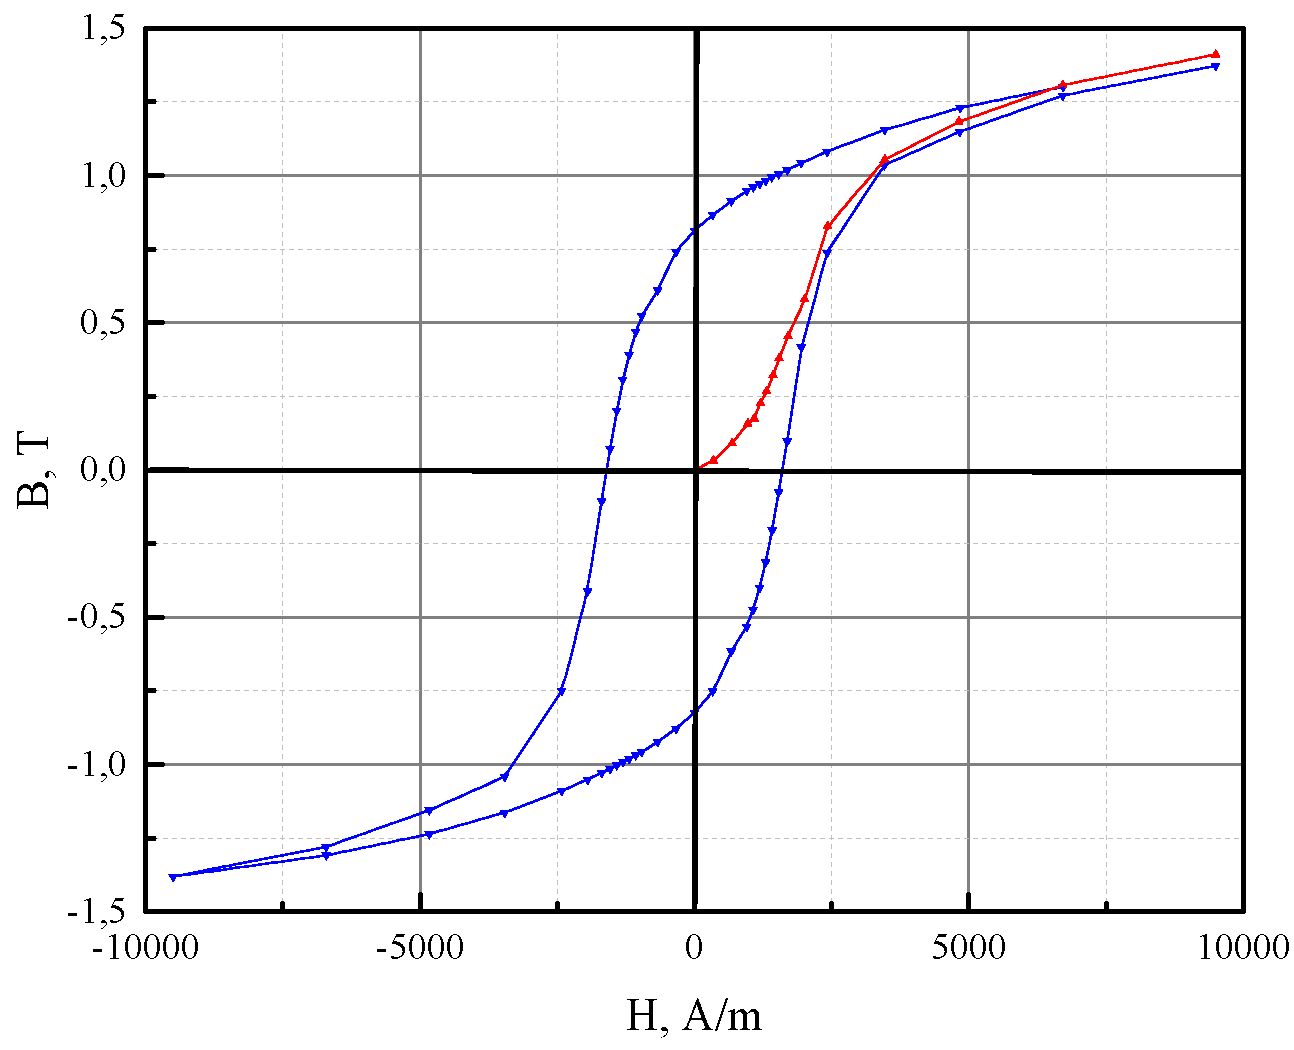
\includegraphics[width=0.7\textwidth]{img/plot.png}
    \caption{Графики зависимости для метода саморепродукции}
    \label{fig:plot}
\end{figure}

\subsection{Результаты измерения решеток}
Сводка результатов измерений в таблице ниже. 

\begin{table}[!ht]
    \centering
    \begin{tabular}{|l|l|l|l|l|l|}
    \hline
        Решетка & 1 & 2 & 3 & 4 & 5 \\ \hline
        Метод I & 0,020$\pm0,003$ & 0,034$\pm0,005$ & 0,060$\pm0,003$ & 0,114$\pm0,004$ & 0,159$\pm0,006$ \\ \hline
        Метод II & - & - & 0,089$\pm0,012$ & 0,140$\pm0,018$  & 0,153$\pm0,022$ \\ \hline
        Метод III & - & - & 0,093$\pm0,011$ & 0,136$\pm0,016$ & 0,170$\pm0,035$ \\ \hline
    \end{tabular}
\end{table}

Можно заметить, что наиболее крупная решетка имеет наиболее близкие друг к другу результаты, в то время, как значения для остальных отличаются при вычислении разными методами. Численная погрешность меньше всего при измерениях первым методом. Отметим, что первый метод также оказался единственным, применимым для измерения периодов мелких решеток.

\subsection{Исследование миры}
В установку предыдущего пункта вместо кассеты с решетками вставлена мира. Аналогичным образом, тремя методами измерены параметры решетки №25, затем №20. Поскольку все вычисления совершенно аналогичны предыдущим пунктам, приведём лишь результаты.

\begin{table}[!h]
    \centering
    \begin{tabular}{|l|l|l|}
    \hline
        Решётка миры & №20. d, см & №25. d, см \\ \hline
        Метод I & 0,039$\pm0,004$ & 0,051$\pm0,005$ \\ \hline
        Метод II & 0,049$\pm0,008$ & 0,063$\pm0,012$ \\ \hline
        Метод III & 0,089$\pm0,013$ & 0,117$\pm0,017$ \\ \hline
    \end{tabular}
\end{table}

Заметим, что результаты последнего метода сильнее всего отличаются от остальных. Погрешность измерений так же, как и в опытах с решёткам, оказалась наименьшей при измерении параметров простраственного спектра. 

\section{Выводы}
В работе мы изучили саморепродукцию и применили его к измерению периодов дифракционных решеток. Параметры данных периодических структур измерены двумя дополнительными методами (по спектру и по увеличенному изображению через линзу). Дополнительные методы измерения дали совпадающие по порядку результаты, однако сходятся сточностью до коэффициента с остальными методами. Результаты измерений и их сравнение представлены в таблицах выше. 

Явления саморепродукции позволило довольно точно оценить параметры решёток по порядку величины, однако наиболее результативным оказался метод измерения пространственного спектра.

\end{document}